\documentclass{beamer}
\usetheme{CambridgeUS}

\usepackage{tikz,pgfplots}
\usepackage{amsmath,amssymb}
\usepackage{xcolor}
\usepackage{graphicx}
\usepackage{wasysym}

\title{SIKE - PQC based on isogenies}
\author{Simon Pohmann}
\institute{University of Passau}

\newcommand{\R}{\mathbb{R}}
\renewcommand{\O}{\mathcal{O}}

\begin{document}

\frame{\titlepage}

\begin{frame}
\frametitle{Elliptic Curves}
Let $K$ be a field of characteristic $\neq 2, 3$.
\begin{definition}
    A (possibly nonsmooth) \emph{elliptic curve} $E$ is the zero set
    \begin{equation*}
        \{ (x, y) \ | \ F(x, y) = 0 \} \subseteq \bar{K}^2
    \end{equation*}
    of some irreducible polynomial $F(x, y) = y^2 - x^3 - Ax - B \in K[x, y]$ together with a point $\O = \infty$ at infinity.
\end{definition}
\begin{definition}
    An elliptic curve $E: y^2 = x^3 + Ax + B$ is called smooth, if the discriminant
    \begin{equation*}
        \Delta(E) := -16(27 B^2 + 4 A^3) \neq 0
    \end{equation*}
\end{definition}
\end{frame}

\begin{frame}
\frametitle{Examples}
\begin{minipage}[t]{0.49\textwidth}
    \centering
    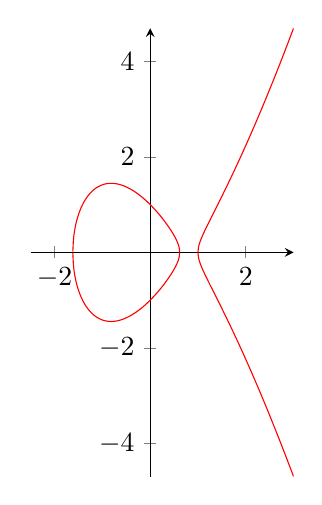
\begin{tikzpicture}
        \begin{axis}[
            axis lines = middle,
            xmin = -2.5,
            axis equal image = true,
            samples = 200
        ]
            \addplot[red, domain=1:3] {sqrt(\x*\x*\x - 2*\x + 1)};
            \addplot[red, domain=1:3] {-sqrt(\x*\x*\x - 2*\x + 1)};
            \addplot[red, domain=-1.618:0.618] {sqrt(\x*\x*\x - 2*\x + 1)};
            \addplot[red, domain=-1.618:0.618] {-sqrt(\x*\x*\x - 2*\x + 1)};
        \end{axis}
    \end{tikzpicture}

    points of $E: x^3 - 2x + 1$ in $\R^2$
\end{minipage}
\begin{minipage}[t]{0.49\textwidth}
    \centering
    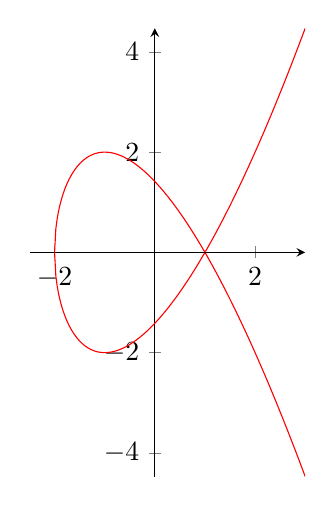
\begin{tikzpicture}
        \begin{axis}[
            axis lines = middle,
            xmin = -2.5,
            axis equal image = true,
            samples = 200
        ]
            \addplot[red, domain=-2:3] {sqrt(\x*\x*\x - 3*\x + 2)};
            \addplot[red, domain=-2:3] {-sqrt(\x*\x*\x - 3*\x + 2)};
        \end{axis}
    \end{tikzpicture}

    points of $E: x^3 - 3x + 2$ in $\R^2$
\end{minipage}
\end{frame}

\begin{frame}
    \frametitle{Coordinate ring}
    \begin{definition}
        Let $E: y^2 = x^3 + Ax + B$ be an elliptic curve. Then 
        \begin{equation*}
            K[E] := K[x, y] / (F), \quad F(x, y) = y^2 - x^3 - Ax - B
        \end{equation*}
        is the \emph{coordinate ring} of $E$.
    \end{definition}
    $f \in K[E]$ are the ``polynomial functions'' defined on $E$
    \begin{equation*}
        (f + gF)(x, y) = f(x, y) + \underbrace{F(x, y)}_{= 0 \ \text{if} \ (x, y) \in E} g(x, y) = f(x, y)
    \end{equation*}
    \begin{definition}
        Let $E: y^2 = x^3 + Ax + B$ be an elliptic curve. Then define the function field $K(E)$ as the quotient field of $K[E]$.
    \end{definition}
\end{frame}

\begin{frame}
    \frametitle{Rational functions - Example}
    Consider $E: y^2 = x^3 - x + 1$ and $f = \frac {(y - 1)(x + 1)} {x(x + 1)} \in K(E)$.
    
    We want to evaluate $f$.
    \begin{itemize}
        \item at $(1, 1)$
        \begin{equation*}
            f(1, 1) = \frac {(1 - 1)(1 + 1)} {1(1 + 1)} = \frac 0 2 = 0
        \end{equation*}
        \item at $(-1, -1)$
        \begin{equation*}
            f(-1, -1) = \frac {(-1 - 1)(-1 + 1)} {-1 (-1 - 1)} = \frac 0 0 \quad \text{\Huge\lightning}
        \end{equation*}
        but in $K(E)$ have
        \begin{equation*}
            \frac {(y - 1)(x + 1)} {x(x + 1)} = \frac {y - 1} {x} \ \Rightarrow \ f(-1, -1) = {-1 - 1} {-1} = 2
        \end{equation*}
    \end{itemize}
\end{frame}

\begin{frame}
    \frametitle{Rational functions - Example}
    Consider $E: y^2 = x^3 - x + 1$ and $f = \frac {(y - 1)(x + 1)} {x(x + 1)} = \frac {y - 1} {x} \in K(E)$.
    
    We want to evaluate $f$.
    \begin{itemize}
        \item at $(0, 1)$
        \begin{equation*}
            f(0, 1) = \frac {1 - 1} {0} = \frac 0 0 \quad \text{\Huge\lightning}
        \end{equation*}
        but in $K(E)$ we have $y^2 = x^3 - x + 1$ so
        \begin{equation*}
            \frac {y - 1} {x} = \frac {(y - 1)(y + 1)} {x(y + 1)} = \frac {y^2 - 1} {x(y + 1)} = \frac {x^3 - x} {x(y + 1)} = \frac {x^2 - 1} {y + 1}
        \end{equation*}
        Hence we define
        \begin{equation*}
            f(0, 1) = \frac {0 - 1} { 1 + 1} = -2
        \end{equation*}
    \end{itemize}
    
    However: $\frac 1 x \in K(E)$ cannot be defined at $(0, 1)$.
\end{frame}

\begin{frame}
    \frametitle{Morphisms}
    Now we consider maps $E \to E'$ for elliptic curves $E, E'$.
    \begin{equation*}
        \phi: E \to E', \quad (x, y) \mapsto (f(x, y), \ g(x, y)) \quad \text{for} \ f, g \in K(E)
    \end{equation*}
    These are called \emph{rational maps} or \emph{morphisms}.
    \vspace{2ex}
    \begin{itemize}
        \item $f(x, y), g(x, y)$ must fulfill the equation of $E'$ for all $(x, y) \in E$
        \\$\Rightarrow \ f, g$ fulfill the equation of $E'$ in $K(E)$ (Hilbert's Nullstellensatz)
        \item Define $\O := (\frac {\neq 0} 0, *) = (*, \frac {\neq 0} 0) = (\frac {\neq 0} 0, \frac {\neq 0} 0)$
        \\$\Rightarrow$ one can always define $f(x, y), \ g(x, y) \in E'$
        \item Write $\phi = [f, g]$
        \item What about $\phi(\O)$?
    \end{itemize}
\end{frame}

\begin{frame}
    \frametitle{Isogenies}
    Let $E, E'$ be elliptic curves.
    \begin{definition}
        A morphism $E \to E'$ that maps $\O$ to $\O$ is called \emph{isogeny}.
    \end{definition}
    \begin{definition}
        A bijective isogeny $E \to E'$ whose inverse is an isogeny is called \emph{isomorphism}.
    \end{definition}
\end{frame}
\end{document}